\section{Graded Assignment 3}\label{sec:graded_assignment_3}

% A full answer and result analysis is expected for task 3 and 4. For task 3 you should include a plot of the pose over time as well as the final estimated landmarks for your choice of parameters, in addition to NEES and NIS over time for the same set of parameters. In task 4 the same plots are expected, where the GPS can be used for ground truth. For both tasks it should be made clear why the parameters were chosen in terms of error metrics, consistency and overall result. Answers and analysis should connect theory and results to the real world, and show your understanding for the problem and solution. Try to connect the results on the simulated data to the results of the read data where and if it is possible. 

An extended Kalman filter was implemented for solving the SLAM problem in MATLAB. Specifically, the EKF-SLAM formulation in this report considers the 2D case, with odometer measurements acting as control input. Furthermore, data association is done with the JCBB algorithm. For the relevant theory behind this EKF-SLAM formulation, consult \cite[p. 185 - 196]{Edmund}.

\subsection{EKF-SLAM on simulated vehicle data set}

\begin{figure}[!htb]
    \centering
    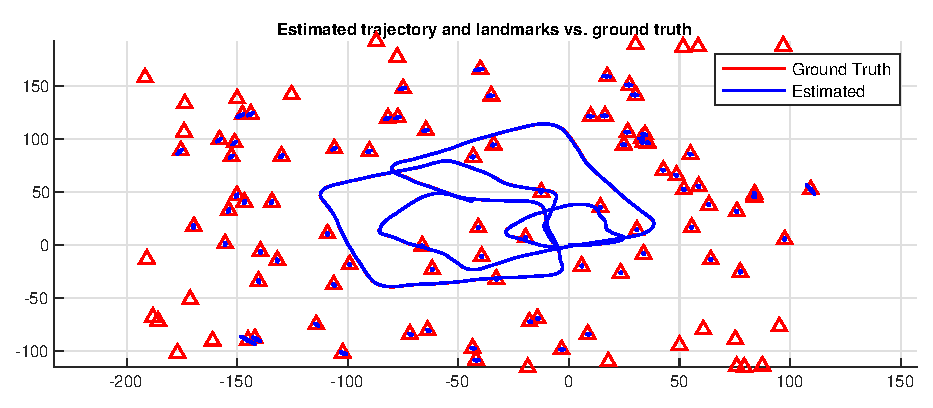
\includegraphics[width=0.8\linewidth]{figures/ga_3/sim_trajectory.eps}
    \caption{Estimated and ground truth pose trajectory and landmarks for simulated vehicle data}
    \label{fig:ga_3_sim_trajectory}
\end{figure}

\begin{figure}[!htb]
    \centering
    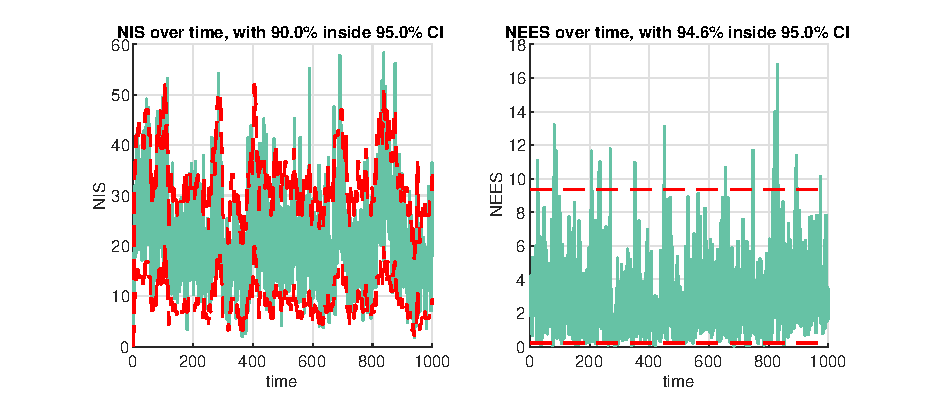
\includegraphics[width=0.8\linewidth]{figures/ga_3/sim_NIS.eps}
    \caption{NIS for simulated vehicle data set with confidence intervals over time}
    \label{fig:ga_3_sim_NIS}
\end{figure}

\subsection{EKF-SLAM on Victoria Park data set}

\begin{figure}[!htb]
    \centering
    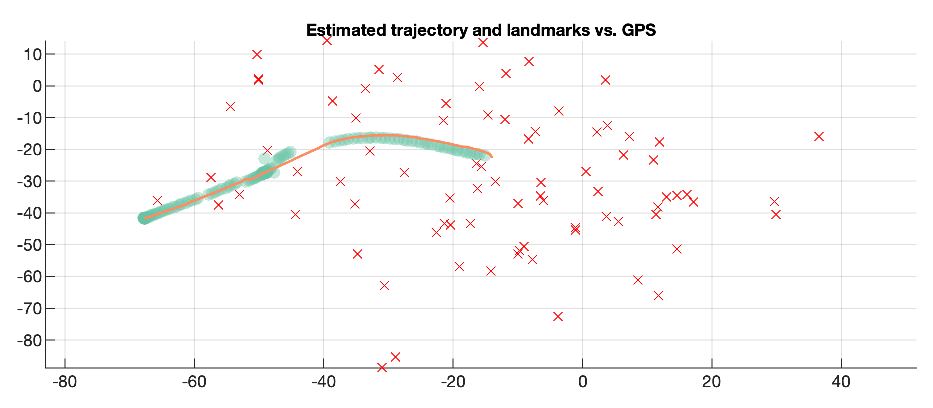
\includegraphics[width=0.8\linewidth]{figures/ga_3/real_trajectory.eps}
    \caption{Estimated pose trajectory, landmarks and GNSS measurements for Victoria Park data set}
    \label{fig:ga_3_real_trajectory}
\end{figure}

\begin{figure}[!htb]
    \centering
    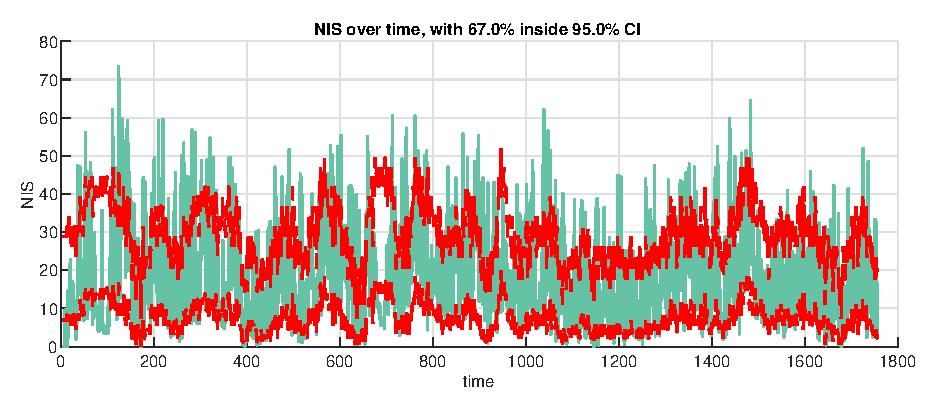
\includegraphics[width=0.8\linewidth]{figures/ga_3/real_NIS.eps}
    \caption{NIS for Victoria Park data set with confidence intervals over time}
    \label{fig:ga_3_real_NIS}
\end{figure}